\chapter[Experiment One: Tag Colour Placement]{Experiment One: Tag Colour Placement}
\label{chap:exp1}
\ifpdf
    \graphicspath{{Chapters/ExperimentOne/Exp1Figs/PNG/}{Chapters/ExperimentOne/Exp1Figs/PDF/}{Chapters/ExperimentOne/Exp1Figs/}}
\else
    \graphicspath{{Chapters/ExperimentOne/Exp1Figs/EPS/}{Chapters/ExperimentOne/Exp1Figs/}}
\fi  

A series of experiments was conducted to explore the potentials and limitations of the interactive tag cloud visualisation tool Taggle. Properties of the enhanced tag cloud features utilised in the system were investigated in two experiments using eye-tracking technology to discover if improvements could be made in user performance for visual search tasks. This chapter details the first experiment, where we investigated manipulation of the tag colour placement in the font and tag background. Research questions and goals for the study are presented in \S\ref{sect:experimentone}. The methodology of the evaluation is detailed from \S\ref{sect:exp1participants} through \S\ref{sect:exp1hypotheses}. Results from the response times and the eye-gaze data analysis are discussed in \S\ref{sect:exp1results}, with threats to the experiment validity considered in \S\ref{sect:threatsexp1}. Finally, results are summarised and conclusions are presented in \S\ref{sect:exp1summary} and \S\ref{sect:exp1conclusions}. 

\section{Foreground or background colour}\label{sect:experimentone}

A special feature of the tag cloud visual encoding in Taggle is the optional use of colour around the tag background instead of the font. This has the benefit of increasing the amount of colour which the user needs to locate in a visual search. Larger areas are better for distinguishing colours (see \S\ref{sect:backgroundcolour} for more details). From a software engineering visualisation perspective, this is important as users of our tag cloud tool will need to deal with correlations between data variables mapped to size and colour. Large datasets, such as those found in software engineering, will inevitably contain small tags. Realising distinguishing colour becomes harder when the tag is smaller, we were interested to find out if increasing the area of colour in a tag could provide a search performance time improvement.

\begin{description}
\item[RQ:]How does altering tag colour placement between font or tag background affect user performance for search tasks? 
\end{description}

Further to this, we wanted to find out if a change in layout or tag size made a difference to any performance change.

Five tag cloud sets consisting of eight tag clouds containing 100 tags each were created within a canvas of $850 \times 650$ pixels (40 tag clouds). The canvas size was determined by screen real estate constraints, while allowing enough room to see layout differences and providing for an average tag length of eight characters across the datasets. Participants saw 32 tag clouds each, plus a trial set of eight tag clouds. 

Each set of tag clouds contained a different colour palette of six colours to minimise the effect of colour combinations having a different impact on visual perception between individual participants. Each colour palette contained a set of six contrasting colours so that we could be reasonably assured participants could distinguish each colour.  Order and size mappings within each tag cloud were varied according to a randomly generated variable. Font sizes were set between 15 pt and 45 pt.

\section{Participants}\label{sect:exp1participants}
We recruited ten University of Canterbury students to participate in the study (age 18\textendash35, all male, with no reported uncorrected vision problems). All had completed, or were completing stage two or three computer science university papers. Participants received a \$20 gift voucher for participating in the study.

\section{Apparatus}\label{sect:apparatusexp1}
Tag clouds were presented on a 17-inch LCD screen with $1280 \times 1024$ pixels. The study was run utilising a Tobii T60 eye-tracking machine attached to the monitor. Eye-gaze data was collected with Tobii Studio 3.2.1 software using a minimum fixation duration of 60 milliseconds. Eye movements of each participant were calibrated to five points before beginning the tasks.

\section{Tag corpora}\label{sect:tagcorpora}
Five tag corpora were developed containing 100 data points each, with a categorical variable containing six categories. These were created from knowledge areas we expected were lesser known to our subjects to minimise bias. Textual data (Table~\vref{table:trialdatasets}) was sourced from real-life datasets retrieved from a variety of sources such as the IUCN list of endangered species\footnote{\url{http://www.iucnredlist.org/}}, Find The Data\footnote{\url{http://www.findthedata.org/}} and the Parliament of Australia\footnote{\url{http://www.aph.gov.au/}}.

\begin{table*}
\centering
\caption{\textit{Datasets used in repetitions}}
\begin{tabular}{|p{3cm}|p{3cm}|p{5cm}|} \hline
\textbf{Repetitions}&\textbf{Dataset}&\textbf{Categorical variable}\\ \hline
Training & Cross country\par team members & Team name\\ \hline
No. 1 & Australian MPs & Political party name\\ \hline
No. 2 & NZ birds & Level of endangerment\\ \hline
No. 3 & US counties & US state\\ \hline
No. 4 & US mines & Mining status\\
\hline\end{tabular}
\label{table:trialdatasets}
\end{table*}

\section{Procedure}

After completing a demographic questionnaire and signing a consent form, five minutes of training describing tag cloud visualisation was given pre-experiment. 

Participants were shown sets of tag clouds varying colour placement, size, and layout, with order counter-balanced using a Latin square design. Each set of tag clouds related to a particular tag corpus, where the target tag was identical for each cloud. Before each set of clouds was displayed, a short text was displayed explaining the scenario and naming a target tag. This text was the same for each cloud set with the scenario adapted to the corresponding tag corpus.  Target tags were selected randomly, with the number of data points within the target category varying between corpus. 

The experiment began with a practice tag cloud set containing eight tag clouds. Following this, four tag cloud sets containing eight tag clouds each (timed trials) were presented (a total of 32 timed trials per participant).

To minimise time and bias, participants performed experiment one and three together, but not experiment two. Overall, participation took 40 to 60 minutes.

\section{Design}
We used a $2 \times 2 \times 2$ experimental design for the following within-subject factors and levels:

\begin{itemize}
	\item Colour placement \{background, foreground\}
	\item Size of tag \{smaller, larger\}
	\item Layout \{spiral, typewriter\}
\end{itemize}

\section{Task} \label{task}
 
Participants completed a visual search task with a random target belonging to a particular category in a tag cloud containing 100 tags. The target was specifically named and there was only one such target within each tag cloud. The number of tags in the target category were distributed across the repetitions (9, 12, 27 and 48). The scenario for the dataset and specific target was described in the instruction screen before the trial, as shown in Figure~\vref{fig:exp1}. 

\begin{figure}
\centering

\begin{subfigure}{.5\textwidth}
  \centering
  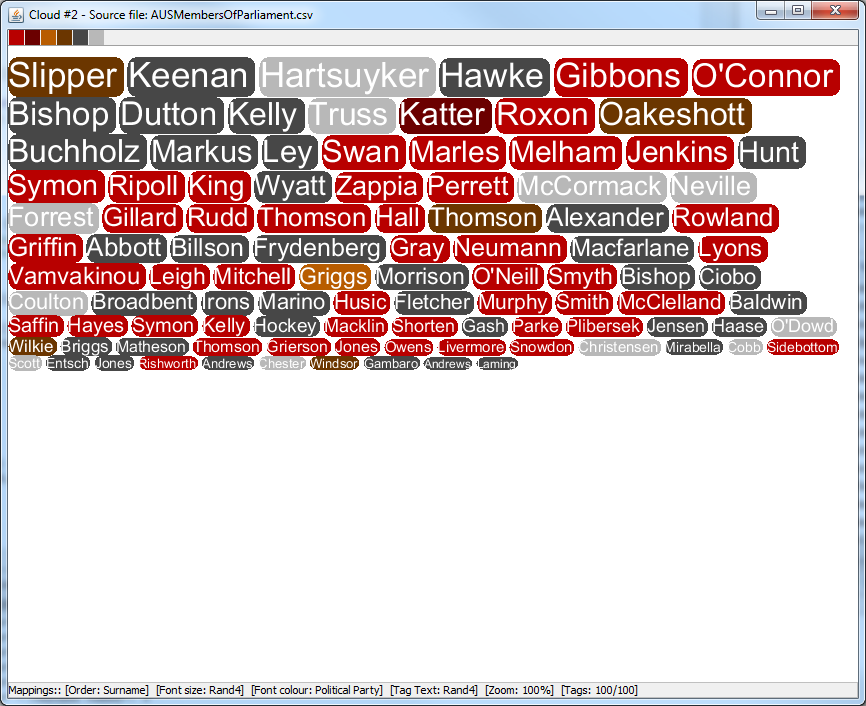
\includegraphics[scale=0.25]{C1S1L2.png}
  \caption{Background colour, typewriter layout}
\end{subfigure}%
\begin{subfigure}{.5\textwidth}
  \centering
  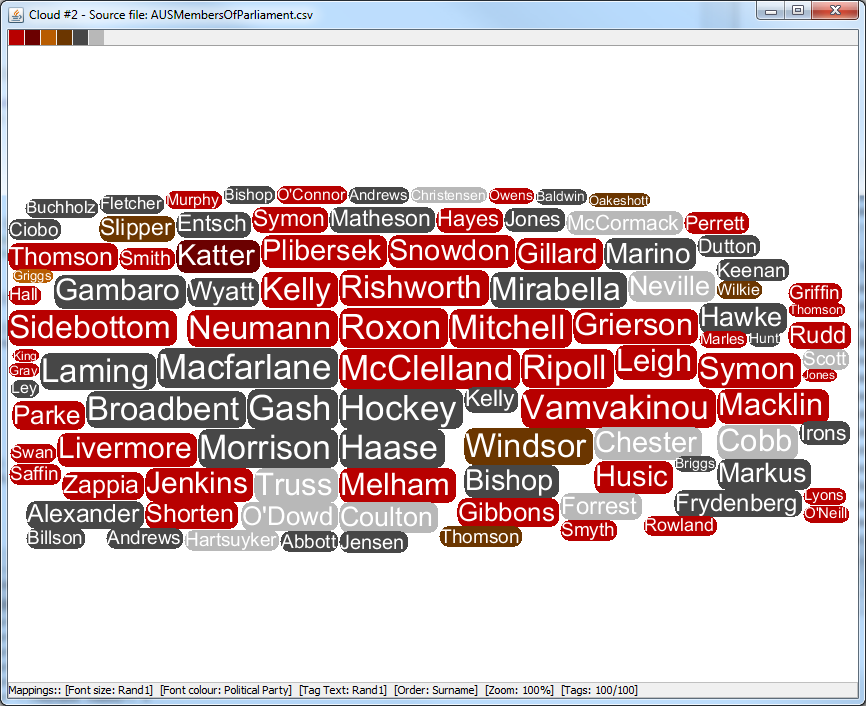
\includegraphics[scale=0.25]{C1S1L1.png}
  \caption{Background colour, spiral layout}
\end{subfigure}
\begin{subfigure}{.5\textwidth}
  \centering
  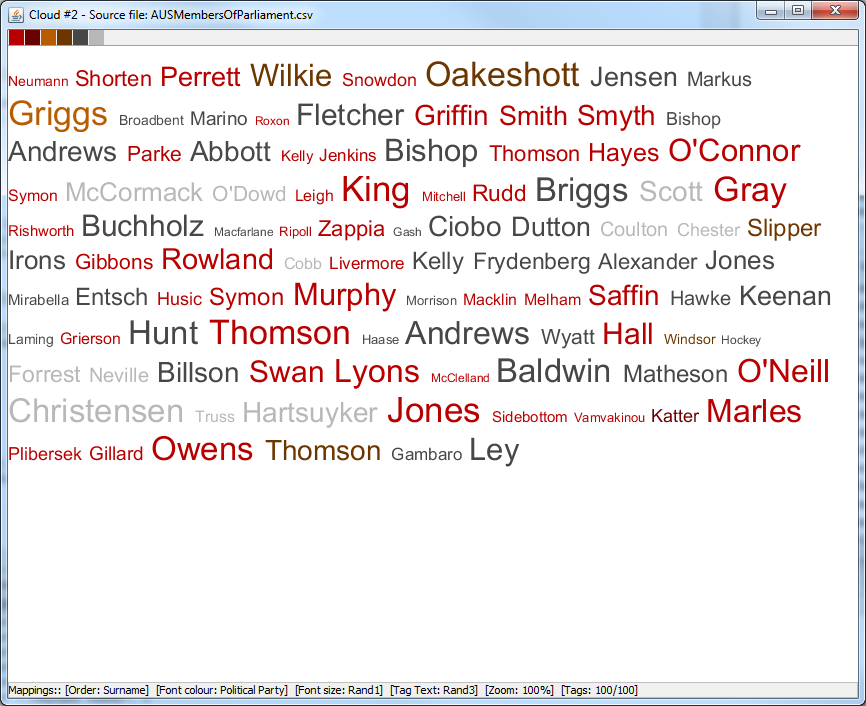
\includegraphics[scale=0.25]{C2S2L2.png}
  \caption{Font colour, typewriter layout}
\end{subfigure}%
\begin{subfigure}{.5\textwidth}
  \centering
  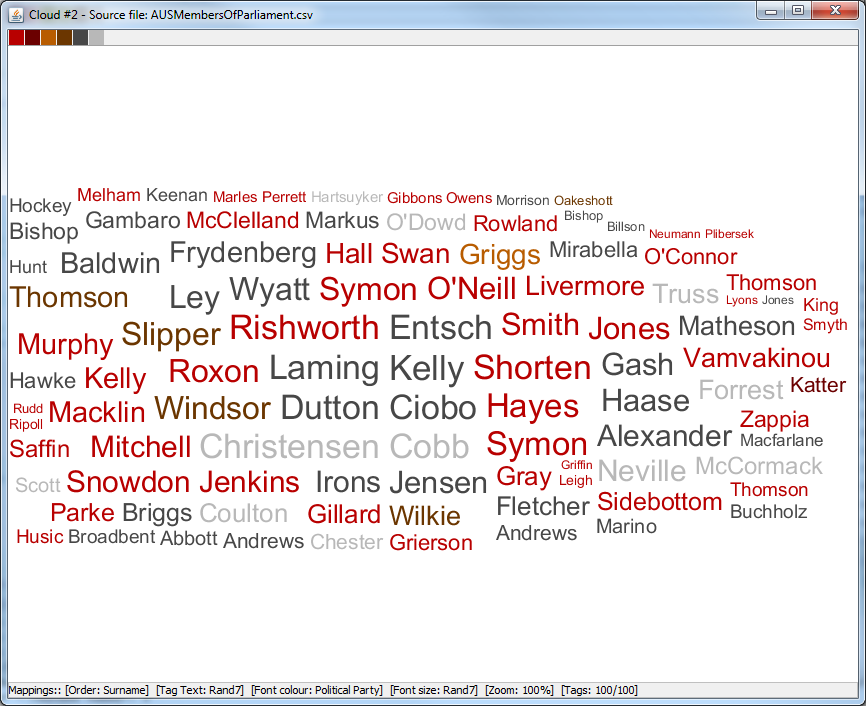
\includegraphics[scale=0.25]{C2S2L1.png}
  \caption{Font colour, spiral layout}
\end{subfigure}
\caption{\textit{Colour and layout in experiment one: You are about to see names of Australian members of parliament from different political parties. Red names belong to the political party 'Australian Labour Party'. Find and click on 'Murphy' from the Australian Labour Party.}}
\label{fig:exp1}
\end{figure}

\section{Measurements}\label{sect:measurements}

The dependent measure was response time (time to first mouse click on target). This was captured by the presentation software between the media first appearing and the user clicking the mouse button on a target. Eye-gaze data was also collected. There was only one target tag in each tag cloud and participants had as much time as they needed to locate the target. There were no incorrect targets selected in the experiment.

\section{Hypotheses} \label{sect:exp1hypotheses}
 
We defined two hypotheses:

\begin{description}
\item[H1:]In general, the larger the area of colour in a colour-coded field, the more easily it can be distinguished \citep[pg 125, ch 4][]{ware04}. Therefore, we hypothesize that \textit{the greater area of colour present in a tag background will lead to faster visual search times for tag background colour than tag foreground colour.}
\item[H2:]\textit{A performance increase for visual search time using tag background colour will be greater for smaller tags than larger tags.}
\end{description}

\section{Results}\label{sect:exp1results}

\subsection{Eye-gaze data analysis} \label{subsect:eyegaze}
The analysis of the eye-tracking data was performed manually, in an exploratory manner looking for typical patterns in the visual search. Previous research \cite{schrammel09b} analysing scan paths in tag clouds has identified two typical search patterns within tag clouds; chaotic scanning (no traceable strategy) and serial scanning (following a zig-zag path). Our exploratory analysis on collected data indicates the introduction of a colour hint in tag searches can alter the search strategy, with the eye scan path focusing on tags with the target colour. Table~\vref{table:searchstrategies} describes the search strategies found in tag clouds in experiment one.

\begin{table*}
\centering
\caption{\textit{Search strategies in tag clouds}}
\begin{tabular}{|p{3cm}|p{5cm}|} \hline
\textbf{Search Type}&\textbf{Gaze Path Description}\\ \hline
Serial scanning & Scanning left to right or right to left successively\\ \hline
Feature search & Fixation clustering around tags with a specific visual feature (colour)\\ \hline
Chaotic search & No fixed pattern\\ 
\hline\end{tabular}
\label{table:searchstrategies}
\end{table*}

Visual feature search was found in all repetitions (which featured different datasets and a different colour palette --- see Figure~\vref{fig:visualfeaturesearch}). However, in datasets containing a larger target category size such as in repetition one (48 tags), some participants used chaotic or serial scanning searches to locate the target. This was also the case in repetition three which had a medium-sized target category (27 tags), but gaze analysis showed participants became confused between the target colour and another closely related colour (light purple and dark purple), increasing the target category size to 47. Figure~\vref{fig:combinationsearch} shows examples where in trial repetitions containing datasets with a larger target category, participants also employed combination searches switching between multiple search strategies.

\begin{figure}[!htb]
\centering
\begin{subfigure}{.5\textwidth}
  \centering
  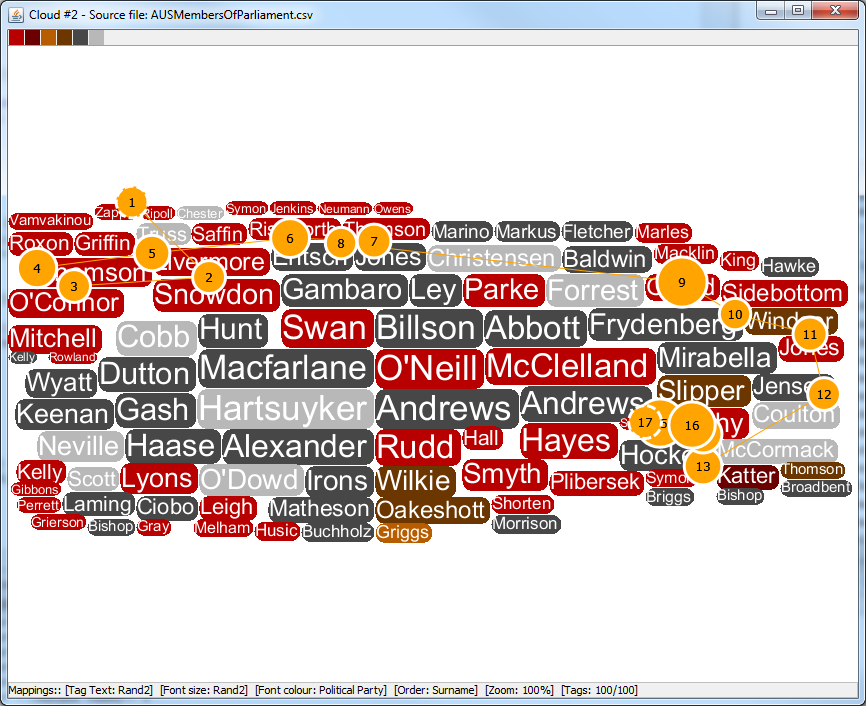
\includegraphics[scale=0.25]{featuresearchgazetrial1.png}
  \caption{Repetition one with red target}
\end{subfigure}%
\begin{subfigure}{.5\textwidth}
  \centering
  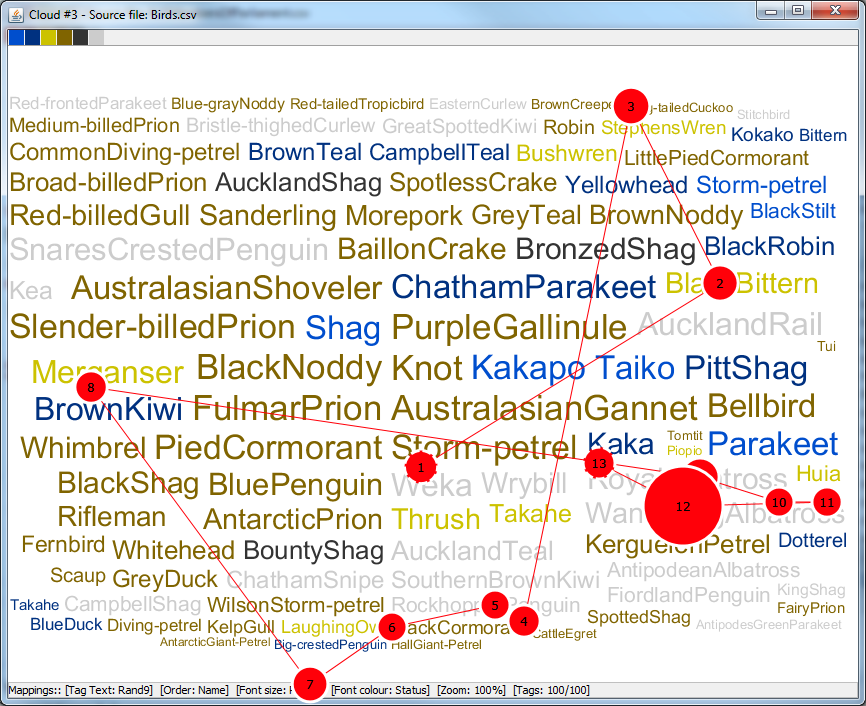
\includegraphics[scale=0.25]{featuresearchgazetrial2.png}
  \caption{Repetition two with yellow target}
\end{subfigure}
\begin{subfigure}{.5\textwidth}
  \centering
  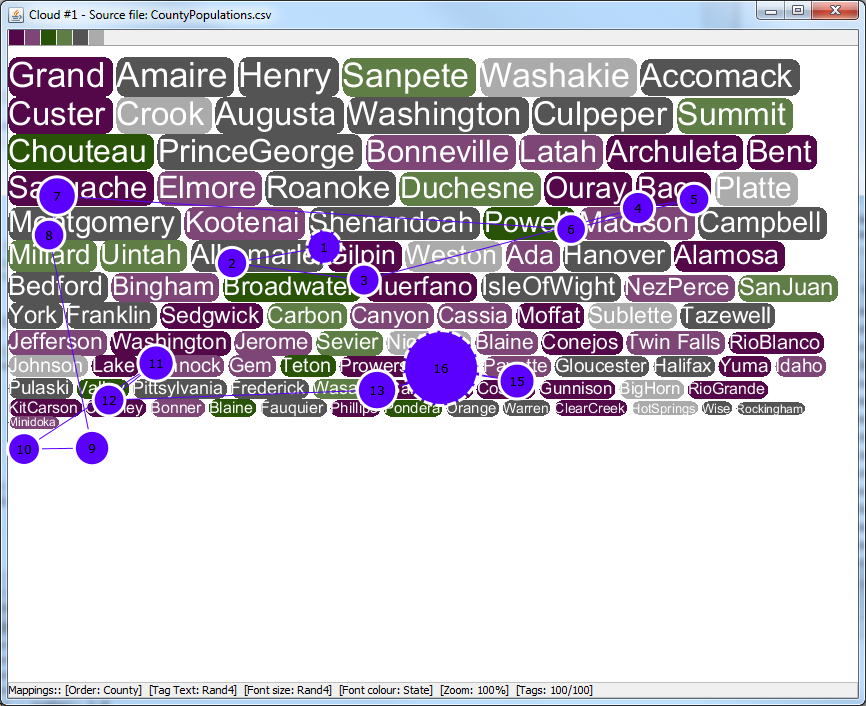
\includegraphics[scale=0.25]{featuresearchgazetrial3.png}
  \caption{Repetition three with purple target}
\end{subfigure}%
\begin{subfigure}{.5\textwidth}
  \centering
  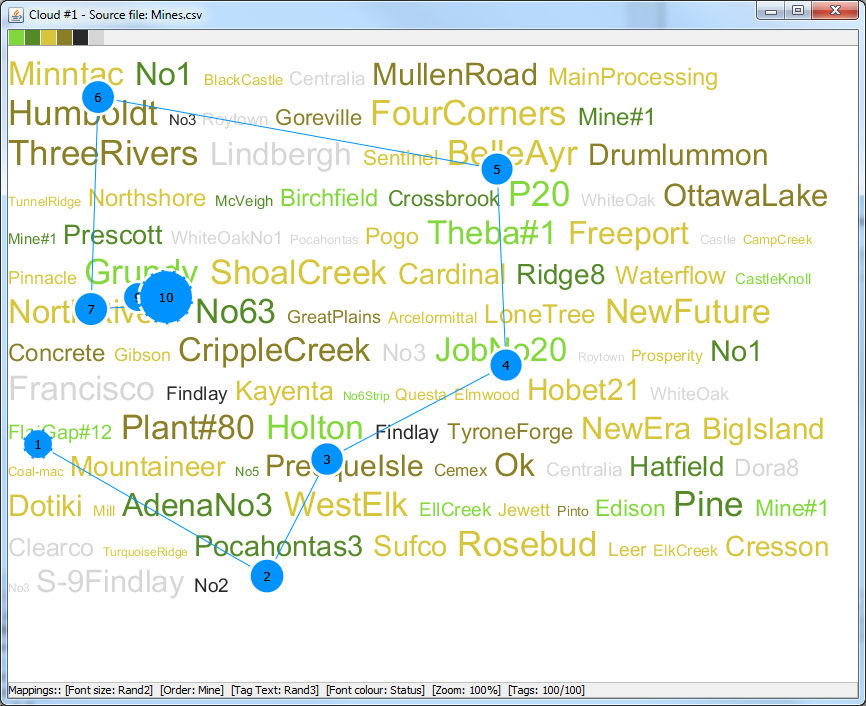
\includegraphics[scale=0.25]{featuresearchgazetrial4.png}
  \caption{Repetition four with green target}
\end{subfigure}
\caption{\textit{Visual feature search with fixation clustering around tags with target colour. Animated visualisations of these examples can be found at \url{http://www.cosc.canterbury.ac.nz/research/RG/svg/taggle/}}}
\label{fig:visualfeaturesearch}
\end{figure}

\begin{figure}[!htb]
\centering
\begin{subfigure}{.5\textwidth}
  \centering
  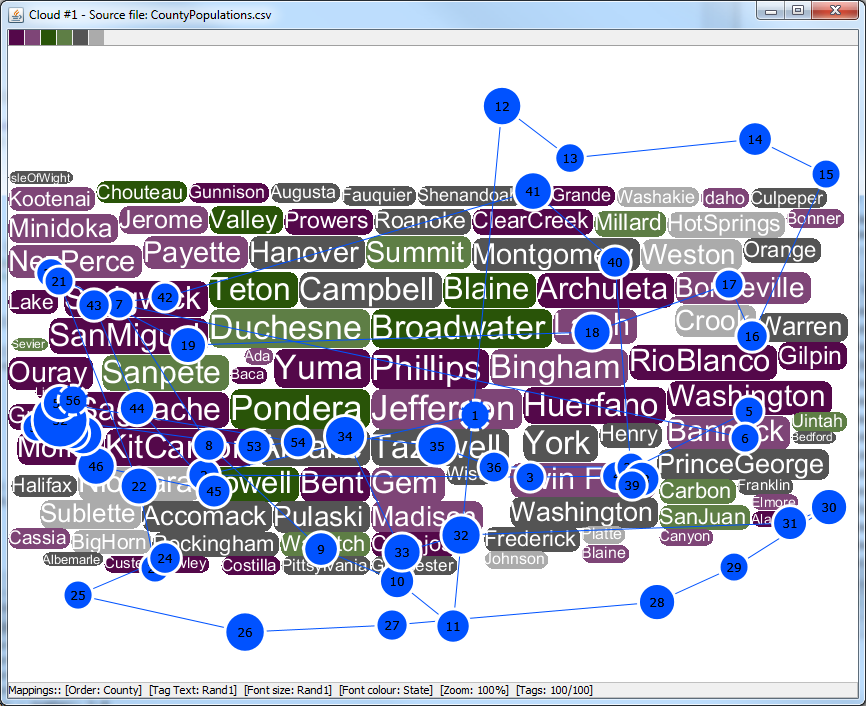
\includegraphics[scale=0.25]{combsearchgazetrial3bgsp.png}
  \caption{Repetition three with dark purple target}
\end{subfigure}%
\begin{subfigure}{.5\textwidth}
  \centering
  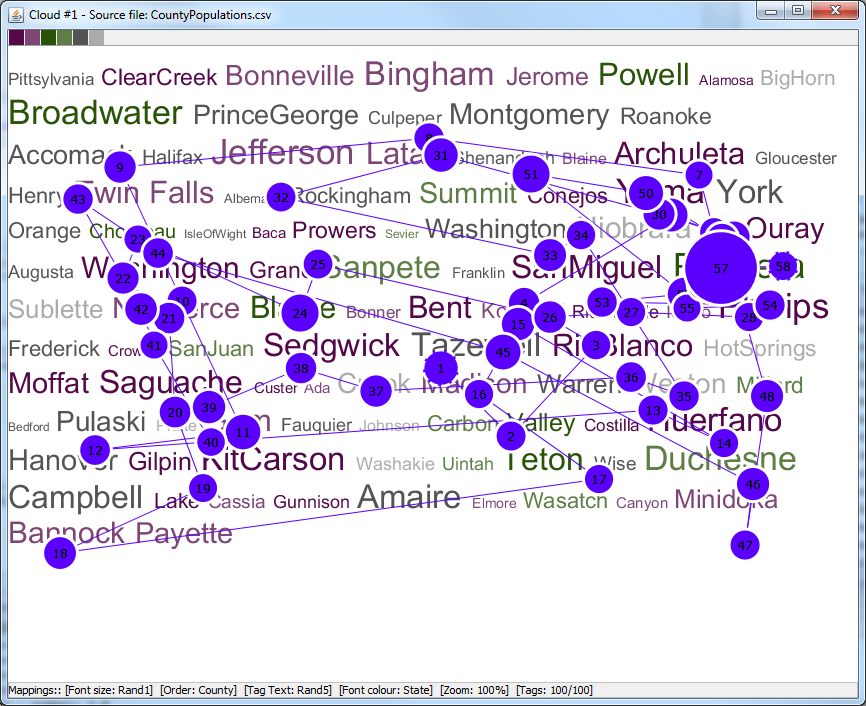
\includegraphics[scale=0.25]{combsearchgazetrial3fgty.png}
  \caption{Repetition three with dark purple target}
\end{subfigure}
\begin{subfigure}{.5\textwidth}
  \centering
  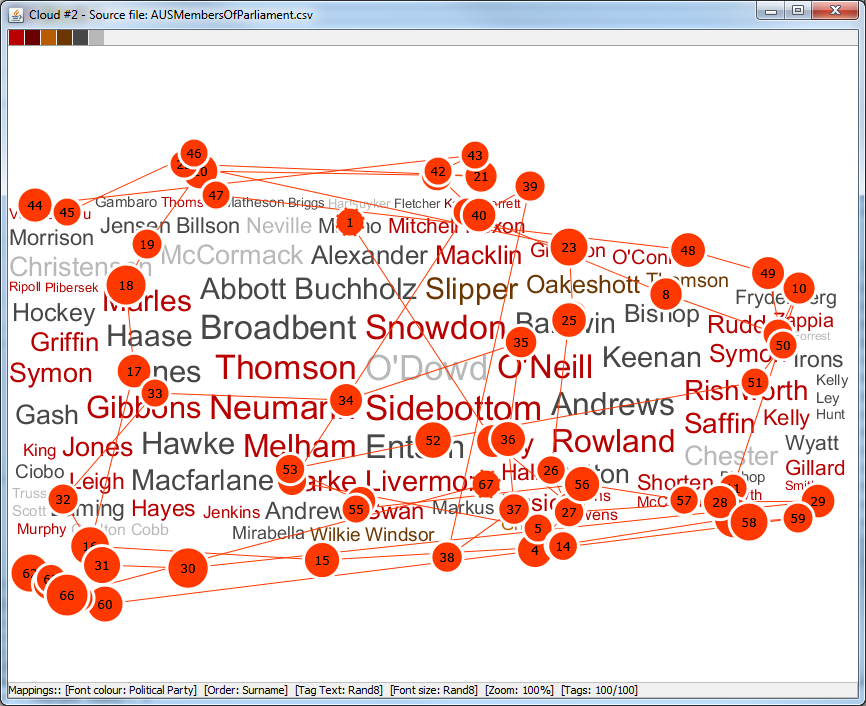
\includegraphics[scale=0.25]{combsearchgazetrial1fgsp.png}
  \caption{Repetition one with red target}
\end{subfigure}%
\begin{subfigure}{.5\textwidth}
  \centering
  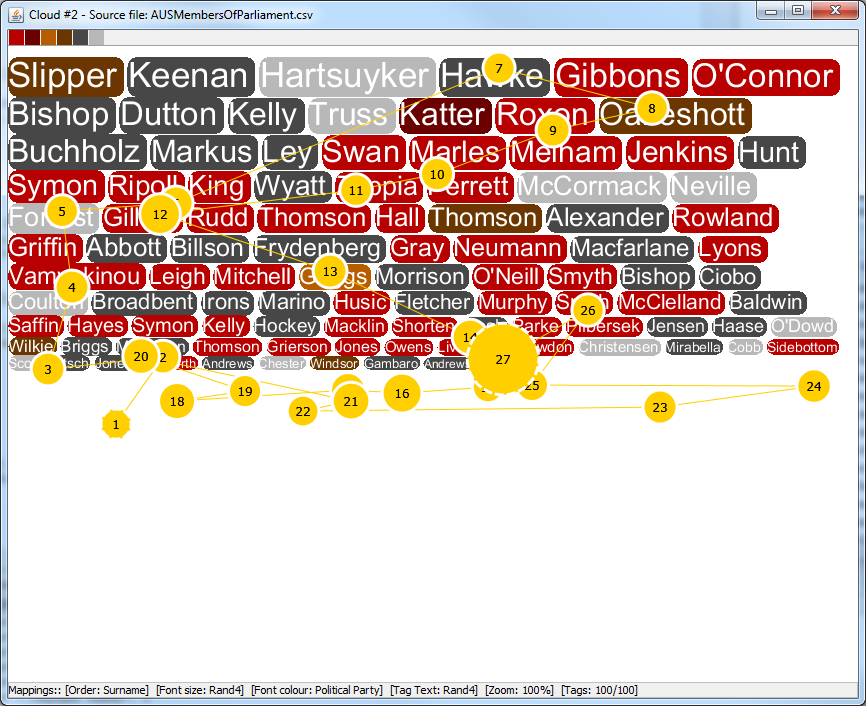
\includegraphics[scale=0.25]{combsearchgazetrial1bgty.png}
  \caption{Repetition one with red target}
\end{subfigure}
\caption{\textit{Visual searches with combinations of chaotic search, serial scanning and fixation clustering around tags with target colour. Animated visualisations of these examples can be found at \url{http://www.cosc.canterbury.ac.nz/research/RG/svg/taggle/}}}
\label{fig:combinationsearch}
\end{figure}

\subsection{Response time} \label{subsect:responsetime}

\begin{figure}[!htb]
	\centering
	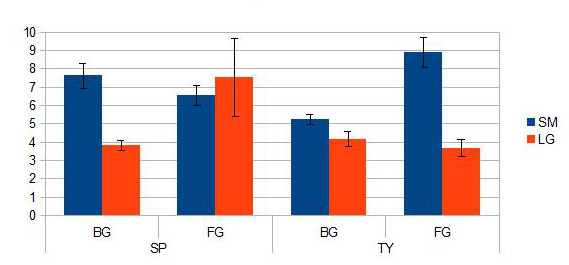
\includegraphics[scale=0.40]{exp1.jpg}
	\caption{\textit{Visual search response time}}
	\label{fig:exp1data}
\end{figure}


Figure~\vref{fig:exp1data} shows response time across colour placement, size and layout and reveals something unexpected in the spiral layout data. While all other colour/layout groups show large tags with a performance advantage over small tags, group foreground colour and spiral layout (FG/SP) show small tags being located faster than large tags. Because of this unexpected and seemingly counter-intuitive result (coupled with the large standard error for that group) the data was carefully screened for the presence of outliers and possible bias.

Data was checked for possible bias in target location between the groups. Target location was assigned randomly to a stimulus. Previous research analysing eye-gaze data for tag clouds has determined initial gaze locations tend towards a central distribution \citep{lohmann09}. It is possible that if the target is positioned further away from a central point that it is found less quickly. We checked to see if randomly placed target positions had resulted in more unfavourable locations for some experimental conditions.

The average location of the first eye fixation across all conditions was calculated. This was close to the stimulus midpoint, but inside the upper left quartile  ---  see Figure~\vref{fig:exp1firstfix}.

\begin{figure}[!htb]
	\centering
	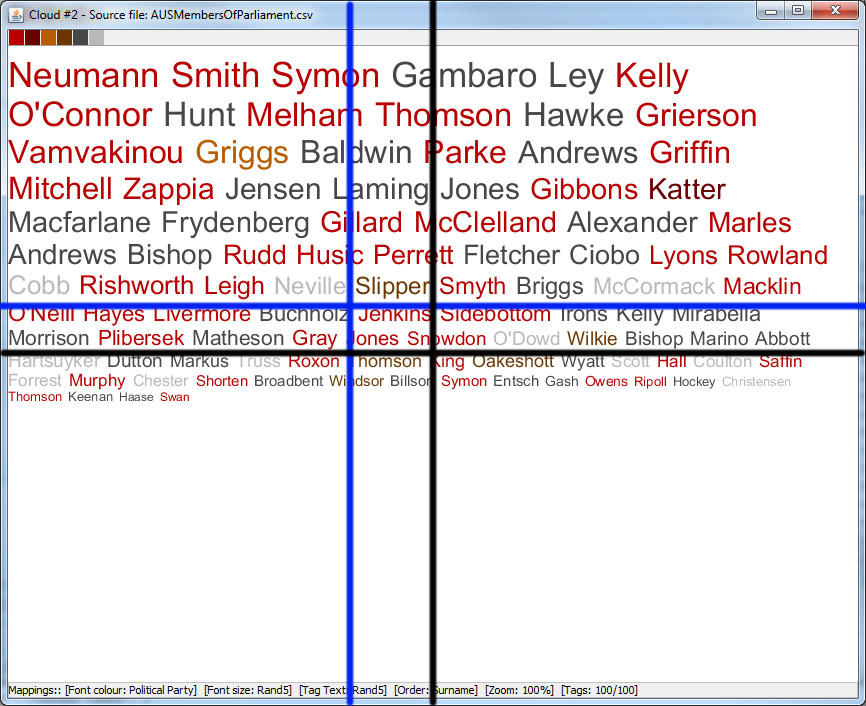
\includegraphics[scale=0.40]{average-firstfixation.png}
	\caption{\textit{Average location of first fixation (blue) and stimulus midpoint (black)}}
	\label{fig:exp1firstfix}
\end{figure}

The distance in pixels between the target tag and average location of first fixation for all stimuli was calculated (4 repetitions $\times$ 8 conditions = 32 visual stimuli). A pictorial representation of a subset of these can be seen in Figure~\vref{fig:fixationdataexp1} where a) shows a favourably located target and b) shows a mildly unfavourably located target (representations of all 32 visual stimuli can be found in Appendix~\ref{appdx:eyegaze}). Average distance to first fixation (Figure~\vref{fig:fixationsexp1}) can be compared with response time results (Figure~\vref{fig:exp1data}) . Response times and average location don't match in the FG/SP condition. Although large tags are more favourably located than small tags, the small tags were found more quickly.

\begin{figure}[h!]
\centering
\begin{subfigure}{.5\textwidth}
  \centering
  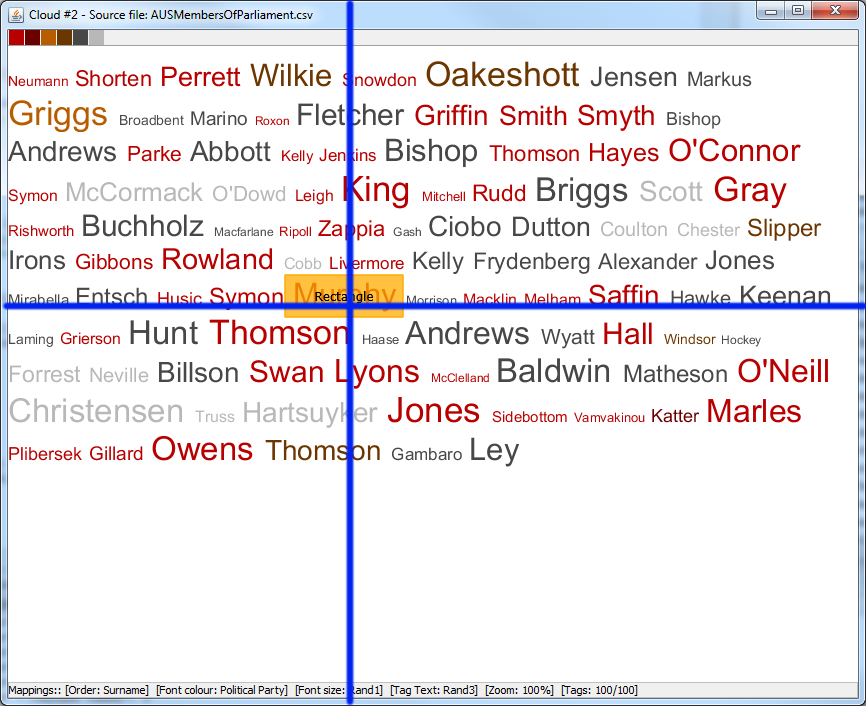
\includegraphics[scale=0.25]{C2S2L2fixation.png}
  \caption{}
\end{subfigure}%
\begin{subfigure}{.5\textwidth}
  \centering
  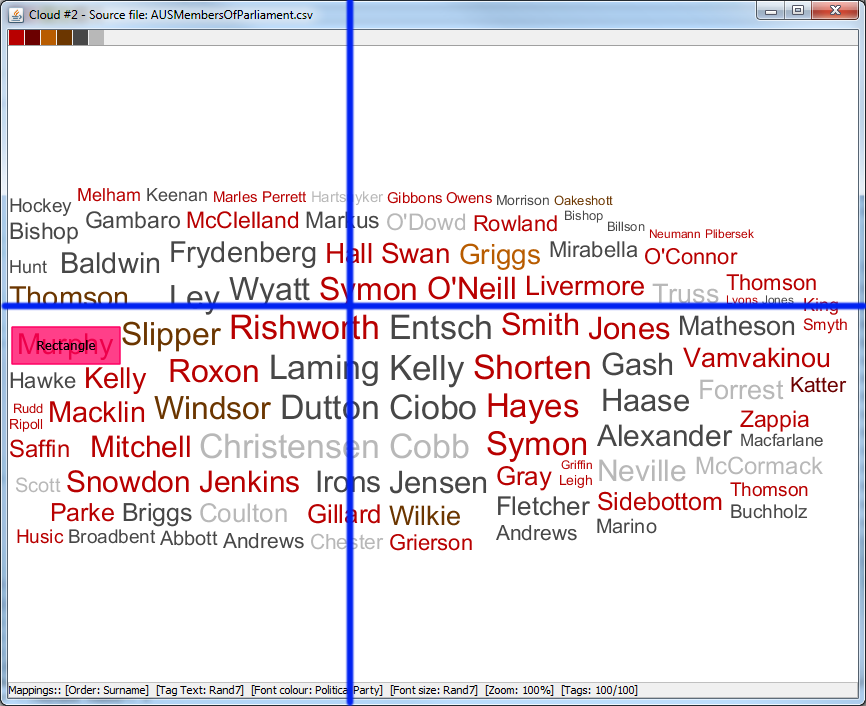
\includegraphics[scale=0.25]{C2S2L1fixation.png}
  \caption{}
\end{subfigure}
\caption{\textit{Foreground colour with large target, typewriter and spiral layout}}
\label{fig:fixationdataexp1}
\end{figure}

\begin{figure}[h!]
	\centering
       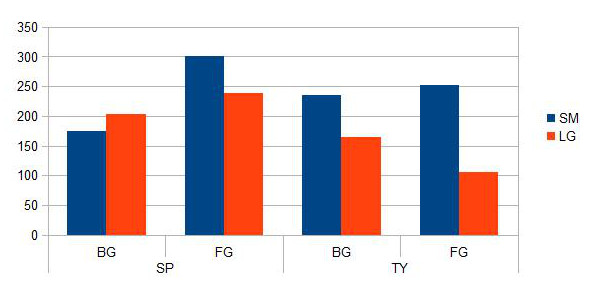
\includegraphics[scale=0.40]{fixations.jpg}
       \caption{\textit{Average distance in pixels to first fixation}}
       \label{fig:fixationsexp1}
\end{figure}


For each condition in each repetition one of four categories for location was assigned; Favourable, Mildly Favourable, Mildly Unfavourable, Unfavourable. Assignation to location category was based on whether the distance was above/below median or 1st and 3rd quartile fixation values (see Table~\vref{table:locationsexp1}).

\begin{table*}
\centering
\caption{\textit{Target location favourableness per condition and repetition}}
\begin{tabular}{|p{2cm}|p{2.5cm}|p{2.5cm}|p{2.5cm}|p{2.5cm}|} \hline
\textbf{Stimulus}&\textbf{R1}&\textbf{R2}&\textbf{R3}&\textbf{R4}\\ \hline
BG/SM/SP&Mildly favourable&Mildly favourable&Mildly\par unfavourable&Mildly favourable\\ \hline
BG/SM/TY&Favourable&Unfavourable&Favourable&Unfavourable\\ \hline
BG/LG/SP&Unfavourable&Unfavourable&Favourable&Favourable\\ \hline
BG/LG/TY&Mildly\par unfavourable&Favourable&Mildly favourable&Mildly favourable\\ \hline
FG/SM/SP&Unfavourable&Unfavourable&Mildly\par unfavourable&Mildly\par unfavourable\\ \hline
FG/SM/TY&Mildly\par unfavourable&Favourable&Unfavourable&Unfavourable\\ \hline
FG/LG/SP&Mildly\par unfavourable&Mildly favourable&Mildly\par unfavourable&Mildly\par unfavourable\\ \hline
FG/LG/TY&Favourable&Mildly\par unfavourable&Favourable&Mildly favourable\\ \hline
\end{tabular}
\label{table:locationsexp1}
\end{table*}

A large number of outliers (42) were calculated outside of three standard deviations from the condition mean. Outliers did not appear to be greatly related to presentation in repetition groups with mildly unfavourable or unfavourable target locations (59 percent). The greatest factor correlated to the presence of outliers was target category size. Outliers were mostly contained to repetition one and repetition three (90 percent) which used datasets containing categories with a large and medium number of data points  (48 and 27). Outliers were spread fairly evenly across all eight conditions, and spread across all but one participant. Data distribution is positively skewed (see Figure~\vref{fig:exp1box}). This positive skew is a characteristic of response times in general \citep[][]{luce86, zandt00} and visual search response time \citep{palmer11}. 


\begin{figure}[h!]
\centering
\begin{subfigure}{.5\textwidth}
	\centering
	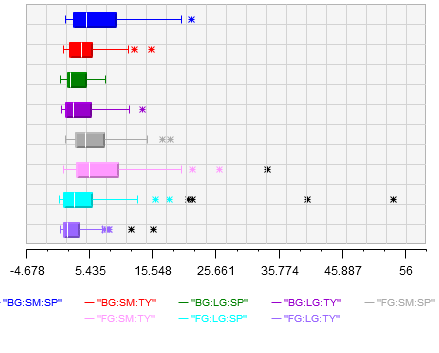
\includegraphics[scale=0.60]{boxplot.png}
\end{subfigure}%
\begin{subfigure}{.5\textwidth}
  \centering
  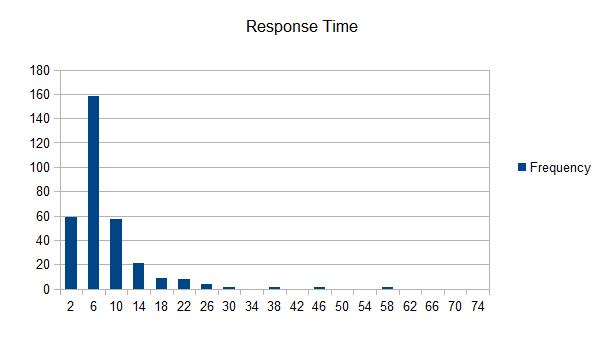
\includegraphics[scale=0.40]{distribution.jpg}
\end{subfigure}
\caption{\textit{Distribution of data}}
\label{fig:exp1box}
\end{figure}


Eye-gaze data for all outlying data points was also analysed.  Analysis of eye-gaze data concluded participants often used the colour visual feature to aid their search for the target tag (\S\ref{subsect:eyegaze}). However, when presented with a larger number of coloured targets such as in trial repetition one, participants appeared to resort to using a random search method or serial scanning to locate the target. It appeared that in repetition three, participants were confused by the presence of two colours  (light and dark purple) which were arguably less strongly contrasting than other pairs. Together these two colour made a large proportion of the dataset (47 tags). Participants searched for the target by either scanning both colours or resorting to using random/serial scanning methods.

Analysis of the response time data revealed the presence of a number of outliers and strongly positively skewed data. Careful examination of eye-tracking data showed outliers were due mostly to a variance in category size which increased the complexity of the task for the participant, rather than experiment procedure or participant error. 

%Then I averaged acoss the four trials to assign a location category for each condition. Average location spanned from mildly favourable to mildly unfavourable across the groups.  You can see the results in Exp1Graphs.ods sheet 'Outlier Analysis' - the background colour of the spreadsheet represents the location category - light blue is favourable to dark blue unfavourable.

%I then added in all the outliers calculated earlier - yellow background are the outliers outside of the interquartile range * 1.5, and pink background are the outliers outside of 3 (positive) standard deviations from the mean. (The yellow outliers are a subset of the pink). Outliers were slightly more likely to appear in groups with mildly unfavourable or unfavourable target locations (59\%). Outliers are pretty much spread evenly across all 8 conditions but are mostly contained to within trial 1 and trial 3 (90\%). Outliers were spread across all but 1 participant.

  %For outliers in T1 there was not much difference whether the target was in a favourable location or not (53\% were in less favourable locations)
 %69\% of outliers in T3 had targets which were in less favourable locations
 %For outliers in other trials (and some of the outliers in T1 and T3) it seemed the participant fixated on the target several times during their search before actually selecting it


\subsection{Significance testing}

A two-way ANOVA with repeated measures on the response times data showed a significant main effect for factor size ($F_{1,39}=52.5$, $p<0.000001$), and a three-way interaction between colour placement, tag size and layout ($F_{1,39}=7.13$, $p<0.011008$). A simple two-way interaction between colour placement and font size within the typewriter layout was revealed during post-hoc analysis. Bonferroni-corrected pairwise comparisons showed tag colour placement in the background produced significantly faster visual search response times than tag cloud foreground placement when the target tag size was small ($t(39)=2.90$, $p<0.0061$). This effect was achieved only when using the typewriter layout. Differences in search response time for large tags with background colour placement and foreground colour placement were not statistically significant in either spiral or typewriter layout. Visual search time for large tags was faster than small tags with an average response time of $t=4.79s$ compared to $t=7.06s$ ($t(159)=3.58$, $p< 0.0005$). All statistical testing was performed applying a logarithm transform so ANOVA data normality assumptions could be met. See Figure~\vref{fig:transformeddata} for normalised response times and interactions for typewriter and spiral layout data.

\begin{figure}[h!]
\centering
\begin{subfigure}{.5\textwidth}
  \centering
  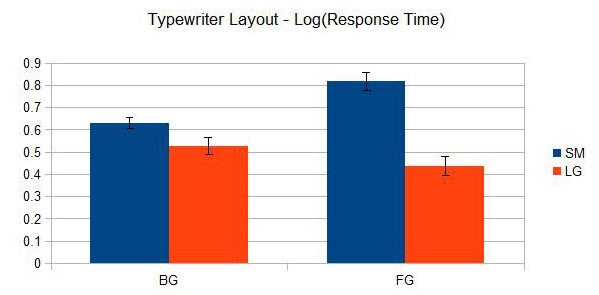
\includegraphics[scale=0.35]{typewriter-log.jpg}
\end{subfigure}%
\begin{subfigure}{.5\textwidth}
  \centering
  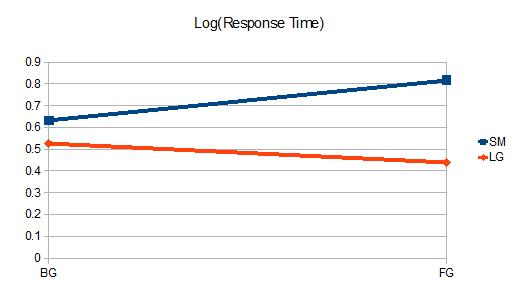
\includegraphics[scale=0.35]{typewriter-log-interaction.jpg}
\end{subfigure}
\begin{subfigure}{.5\textwidth}
  \centering
  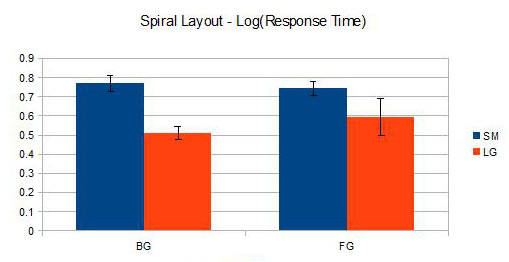
\includegraphics[scale=0.35]{spiral-log.jpg}
\end{subfigure}%
\begin{subfigure}{.5\textwidth}
  \centering
  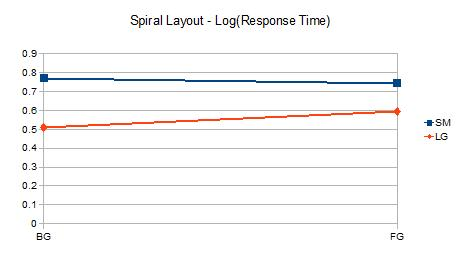
\includegraphics[scale=0.38]{spiral-log-interaction.jpg}
\end{subfigure}
\caption{\textit{Normalised response times and interactions}}
\label{fig:transformeddata}
\end{figure}

\section{Threats to validity}\label{sect:threatsexp1}

Usage of genuine categorical datasets, while realistic, can add challenges. It is possible that the use of real text with long words increasing text size has introduced bias, as this has been shown to have an effect on user perception of tag importance \citep{bateman08}. However, this may be mitigated by the visual search task type as users were not identifying tags of subjective importance, but searching for a specifically named tag. 

Some of the experiment conditions have (averaged across across all stimuli shown) an overall more potentially favourable target location than other conditions (it is unknown how much influence distance to average first fixation point has on search time). This does not appear to have resulted in a pattern in the response times or impacted the conditions where outliers have appeared. 

\section{Summary and discussion}\label{sect:exp1summary}

Analysis of the response time data revealed an unexpected result in foreground colour and spiral layout conditions  ---  small tags were found more quickly than large tags. This is counter-intuitive and also contravening results in previous studies on the effect of font size on user perception in tag clouds (see \S\ref{sect:fontsize} for details of this). Eye-tracking data did not show a bias in target location that might explain this result, as large tags were more favourably placed than small tags for this condition. Careful analysis of outlying data points indicated outlier presence seemed related to target category size, and overall distribution showed a significant positive skew. Therefore, all statistical testing was completed using a logarithm transform so data would conform to statistical testing requirements of normality.

\textbf{H1:} \textit{Placement of colour in the tag background produced faster visual search times than tag foreground colour, but only when searching for small tags, and only when the tag cloud was displayed in a typewriter layout.}  Placement of tag colour made no difference to response time in a tag cloud displayed in a spiral layout. We don't know why the results were different for layouts: whether there is some inherent difference in the way users search for visual targets in a spiral layout, or there was something particular to the spiral layout algorithm used in our experiment. Further close analysis of the eye-tracking data could be performed in the future to explore this further.

\textbf{H2:}\textit{The performance increase seen in typewriter layout for visual search time using tag background colour was only when locating smaller tags and NOT larger tags.} As expected, using a greater area of colour to search for when locating tags was of benefit mostly when searching for tags with smaller sized fonts.

Analysis of eye-tracking data indicates the introduction of a colour hint in tag searches can alter the search strategy from serial scanning or chaotic search methods, to the eye scan path focusing on tags with the target colour. In trial repetitions containing datasets with a larger target category, participants also employed combination searches switching between multiple search strategies.

\section{Conclusion and future work}\label{sect:exp1conclusions}

Our results indicate usage of tag background colour as a data variable field can produce faster visual search response times than foreground colour when the target tag is small. This has implications for designers of tag cloud visualisations. Small tag sizes are inevitable in tag clouds, especially when visualising large datasets. We think providing the background colour option as the default setting in our interactive tag cloud visualisation tool could help users in the following ways: identifying the variables mapped to colour (particularly those displayed with small or iconified tags), and exploring correlations more efficiently between data variables mapped to size and colour. 

This experiment has provided some insight into tag cloud visual search patterns. Varying target category size over repetitions produced some abnormally long response times (outliers) for categories with greater sizes. Eye-tracking data analysis showed when searching for targets in larger sized categories, participants employed combination search methods switching between visual feature search (with colour), serial scanning and chaotic search. 

For future experiments it would be interesting to focus on category size as an experiment factor to further explore eye scanning methods and to discover at what point (such as an overall percentage or specific tag number) participants start producing greater numbers of atypical long response times. Our experiment produced differing results between the two layouts tested, spiral and typewriter. The reasons for this are unclear. Future eye-tracking data analysis or experiments may focus on finding out more about this difference.


% ------------------------------------------------------------------------

%%% Local Variables: 
%%% mode: latex
%%% TeX-master: "../thesis"
%%% End: 

